%\graphicspath{{/home/arbon/Pictures/Screenshots/}} % path to graphics
\graphicspath{{~/Documents/SADT/FirstTask/BaCD}}
\chapter{Работа с ветвлением и оформление кода}

\section{Форк репозитория}

Чтобы сделать форк перейдем к нужному репозитории в GitHub и в верхнем левом
углу нажмем на кнопку "<fork">. На появившейся странице потребуется
ввести имя форка (Рисунок~\ref{3:fig:GitHub:fork}).

\begin{figure}[h!tp]
	\centering
	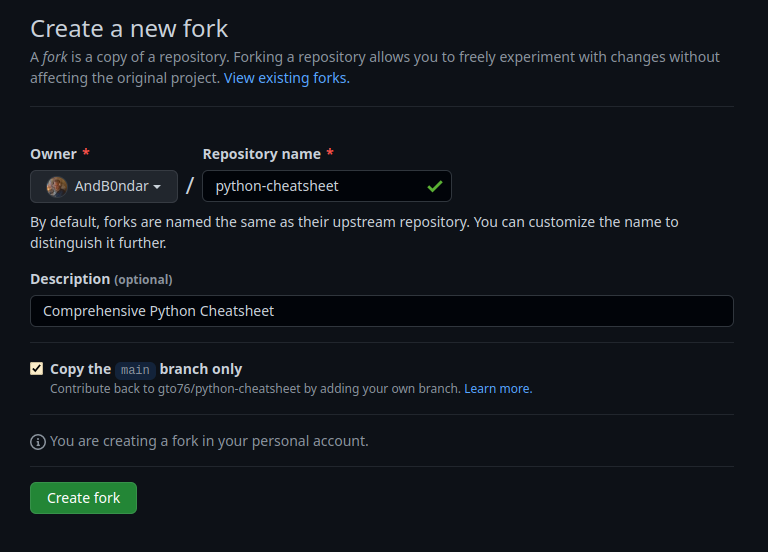
\includegraphics[width=0.7\textwidth]{Screenshot from 2023-02-19 20-37-21.png}
	\caption{Создание форка в GitHub}
	\label{3:fig:GitHub:fork}
\end{figure}

\section{Клонирование форка на локальную машину}

Клонирование репозитория производиться командой:
\texttt{git~clone~<адрес~форка>} (Рисунок~\ref{3:fig:git:fork:clone}).

\begin{figure}[h!tp]
	\centering
	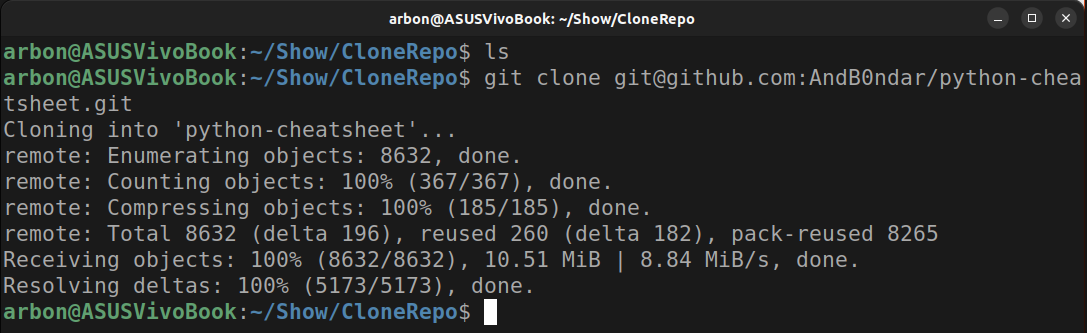
\includegraphics[width=0.8\textwidth]{Screenshot from 2023-02-19 20-56-11.png}
	\caption{Клонирование форка}
	\label{3:fig:git:fork:clone}
\end{figure}

\section{Создание двух веток}

Создание новой ветки производиться командой:
\texttt{git~branch~<имя~ветки>} (Рисунок~\ref{3:fig:git:branch}).

\begin{figure}[h!tp]
	\centering
	
\includegraphics[width=0.9\textwidth]{Screenshot from 2023-02-19 20-59-52.png}
	\caption{Создание двух веток}
	\label{3:fig:git:branch}
\end{figure}

\section{Коммиты}
Теперь создадим по три коммита в каждой ветке. Для этого воспользуемся
командой: \texttt{git commit -am "текст коммита"}, которая добавит в индекс
все изменения в индекс и сделате коммит. Изменения проиллуюстрированы
на рисунках~\ref{3:fig:git:branch:1:commits}-\ref{3:fig:git:branch:2:commits}.

\begin{figure}[h!tp]
	\centering
	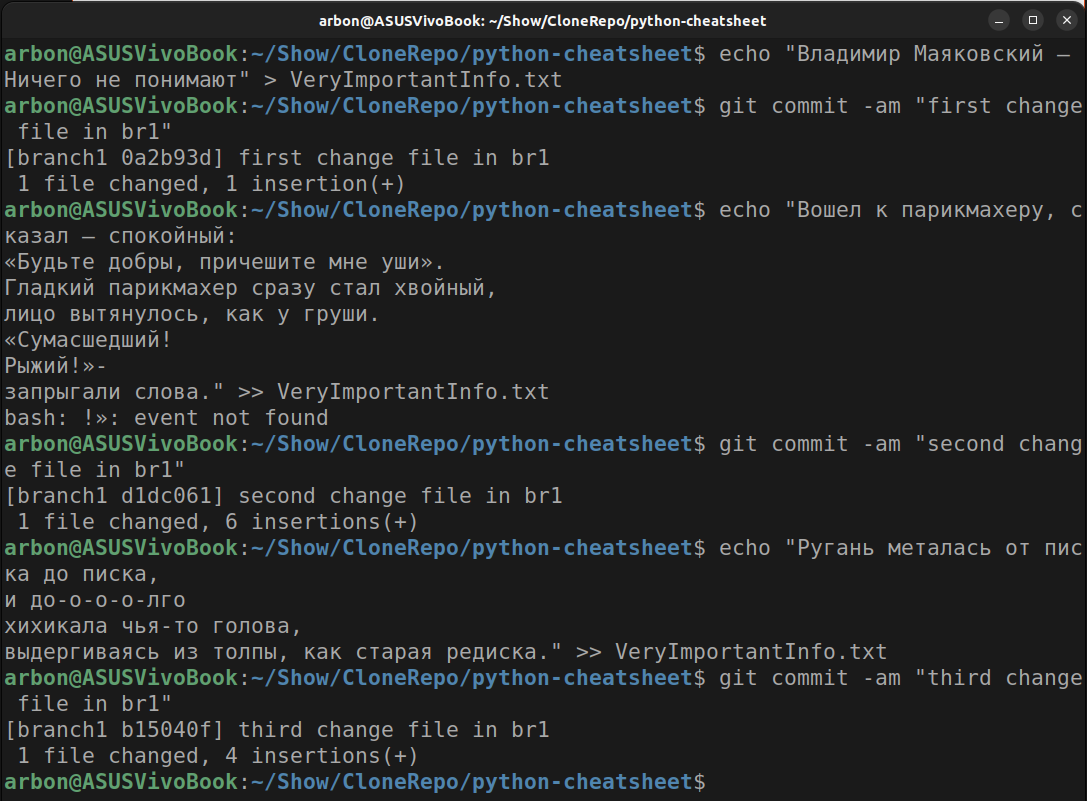
\includegraphics[width=0.8\textwidth]{Screenshot from 2023-02-19 21-16-40.png}
	\caption{Создание трех коммитов в ветке branch1}
	\label{3:fig:git:branch:1:commits}
\end{figure}
\begin{figure}[h!tp]
	\centering
	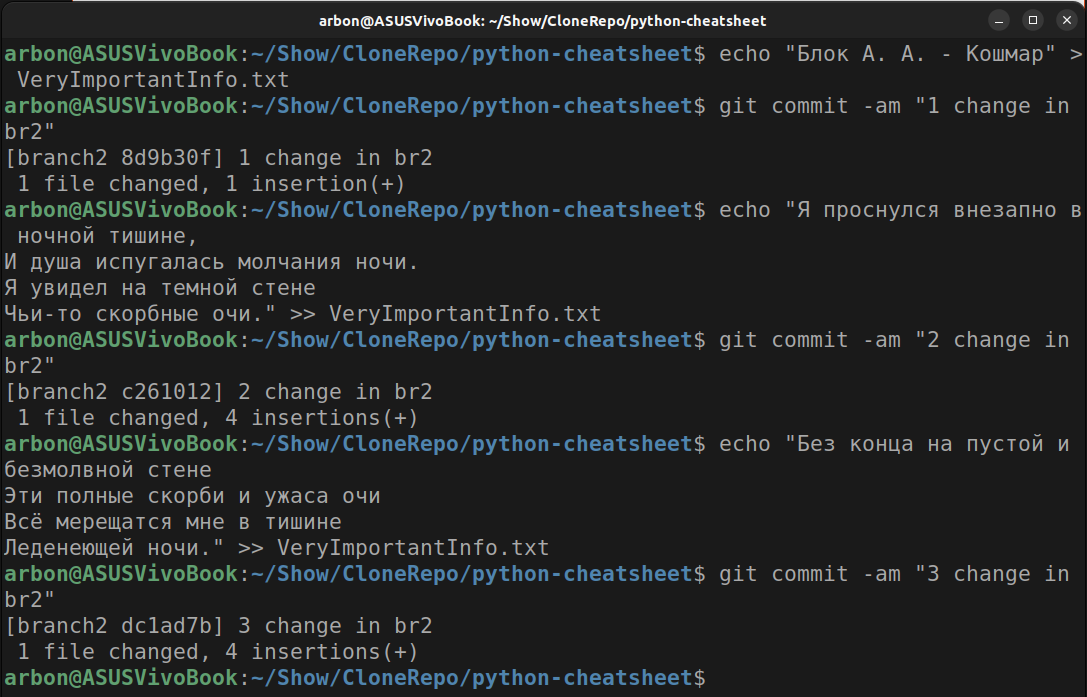
\includegraphics[width=0.8\textwidth]{Screenshot from 2023-02-19 21-21-50.png}
	\caption{Создание трех коммитов в ветке branch2}
	\label{3:fig:git:branch:2:commits}
\end{figure}

\section{Слияние веток}
\label{3:lb:git:merge:conflict}
Чтобы слить ветку А в ветку Б используется команда: \texttt{git merge Б}.
Если при силянии появился конфликт и git не смог автоматически разрешить его,
то необходимо открыть файл с конфилктом в любом из редакторов и исправть
выделенный участок. Затем останеться выполнить команду \texttt{git commit}
для создания коммита слияния. 

Эти действия проиллуюстрирован на рисунке~\ref{3:fig:git:merge}.

\begin{figure}[h!tp]
	\centering
	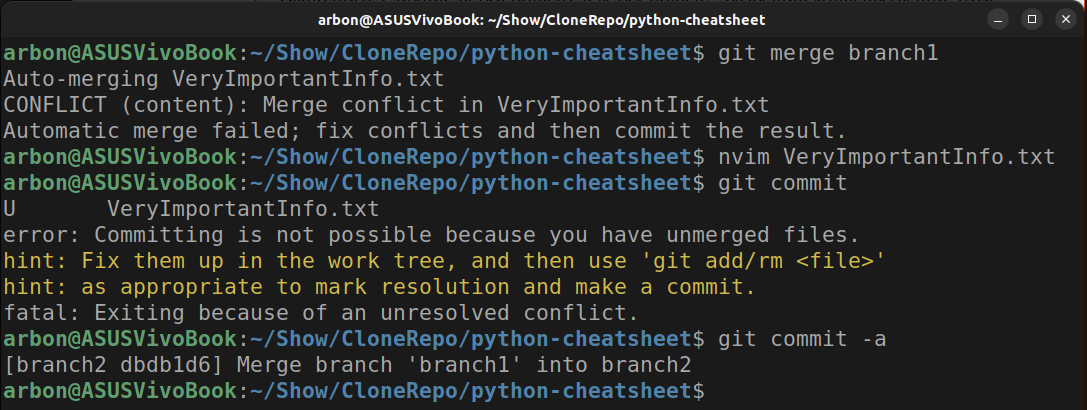
\includegraphics[width=0.8\textwidth]{Screenshot from 2023-02-19 21-48-53.png}
	\caption{Слиянине ветки branch1 в ветку branch2}
	\label{3:fig:git:merge}
\end{figure}

\section{Отправка всех изменений}
Чтобы отправить все изменения введем команду
\texttt{git~push~origin~<название~ветки>} для каждой ветки
(Рисунок~\ref{3:fig:git:push:all}).

\begin{figure}[h!tp]
	\centering
	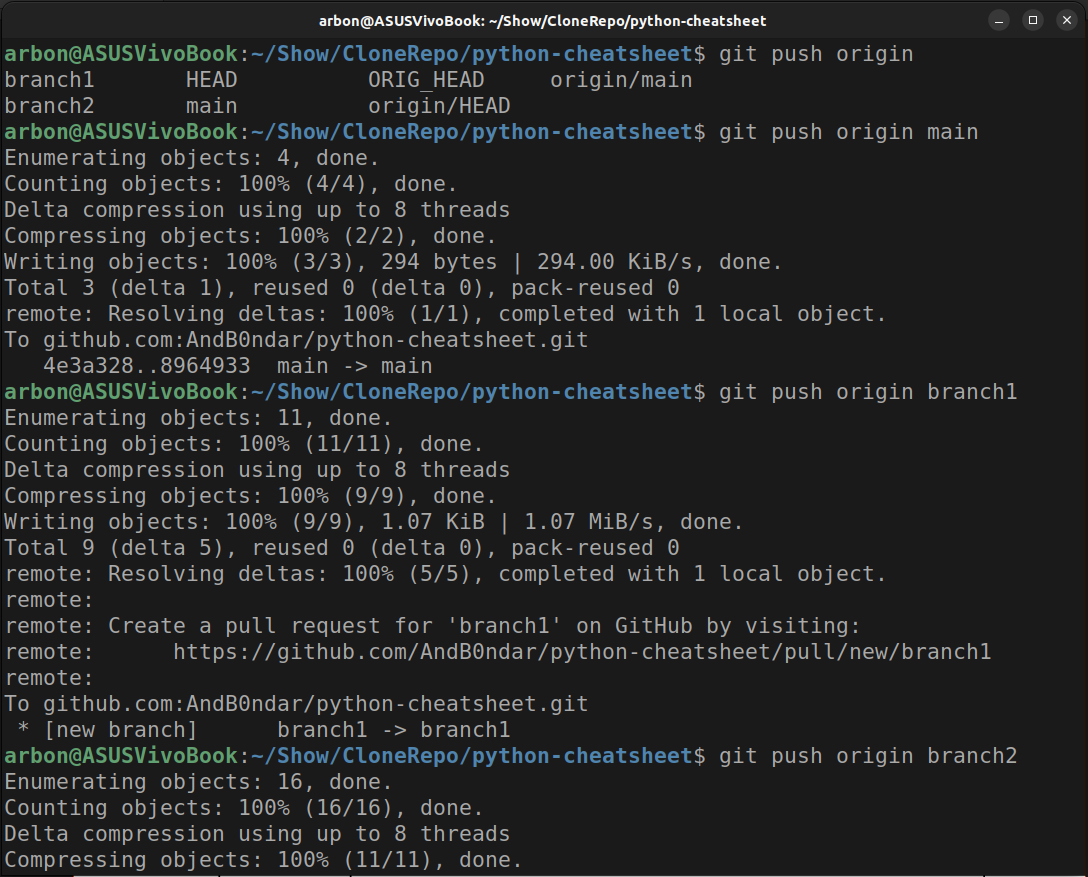
\includegraphics[width=0.8\textwidth]{Screenshot from 2023-02-19 22-00-30.png}
	\caption{Отправка всех изменений}
	\label{3:fig:git:push:all}
\end{figure}

\section{Еще три коммита}
Проведем еще три коммита в ветку branch1 (Рисунок \ref{3:fig:git:3commits}).

\begin{figure}[h!tp]
	\centering
	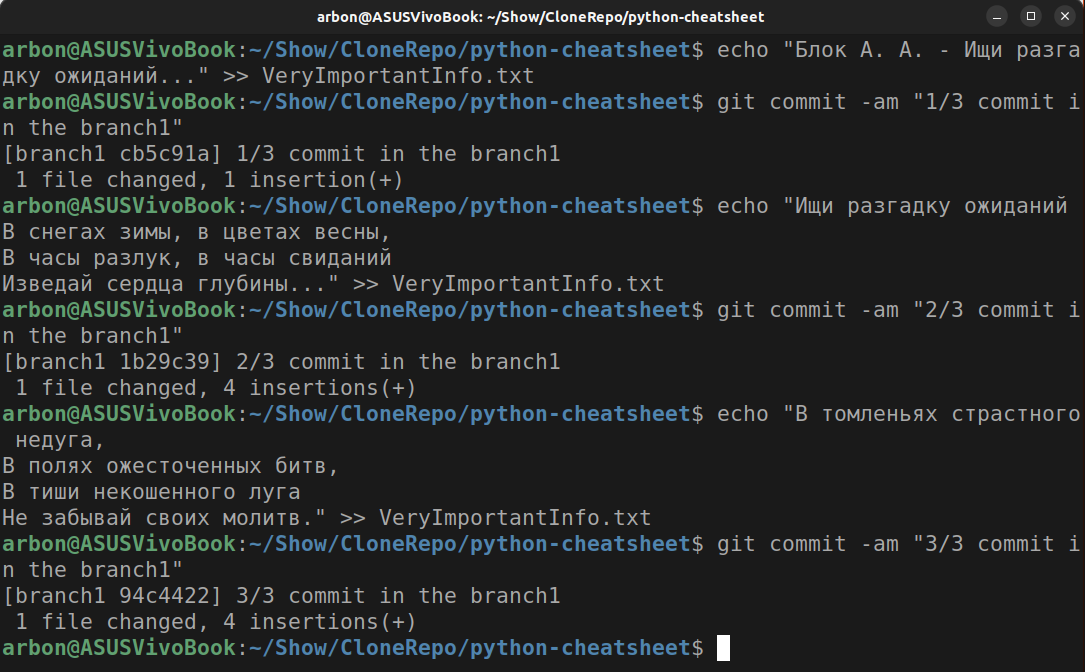
\includegraphics[width=0.6\textwidth]{Screenshot from 2023-02-20 11-58-20.png}
	\caption{Создание еще трех коммитов}
	\label{3:fig:git:3commits}
\end{figure}

\section{Еще одно клонирование репозитория}
Склонируем репозиторий еще раз в другую директорию
(Рисунок~\ref{3:fig:git:clone:new}).

\begin{figure}[h!tp]
	\centering
	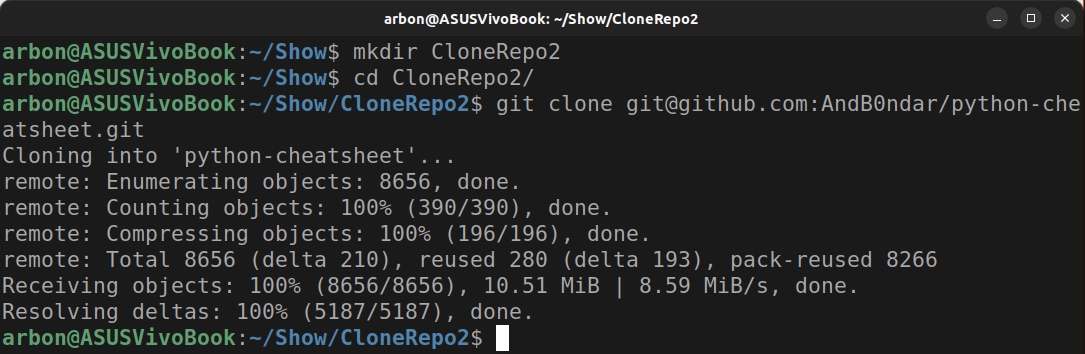
\includegraphics[width=0.8\textwidth]{Screenshot from 2023-02-20 12-01-42.png}
	\caption{Новый клон репозитория}
	\label{3:fig:git:clone:new}
\end{figure}

\section{Добавление коммитов в новый репозиторий}
В новом клоне репозитории сделаем 3 коммита в ветку branch1
(Рисунок~\ref{3:fig:git:clone:new:commits}).

\begin{figure}[h!tp]
	\centering
	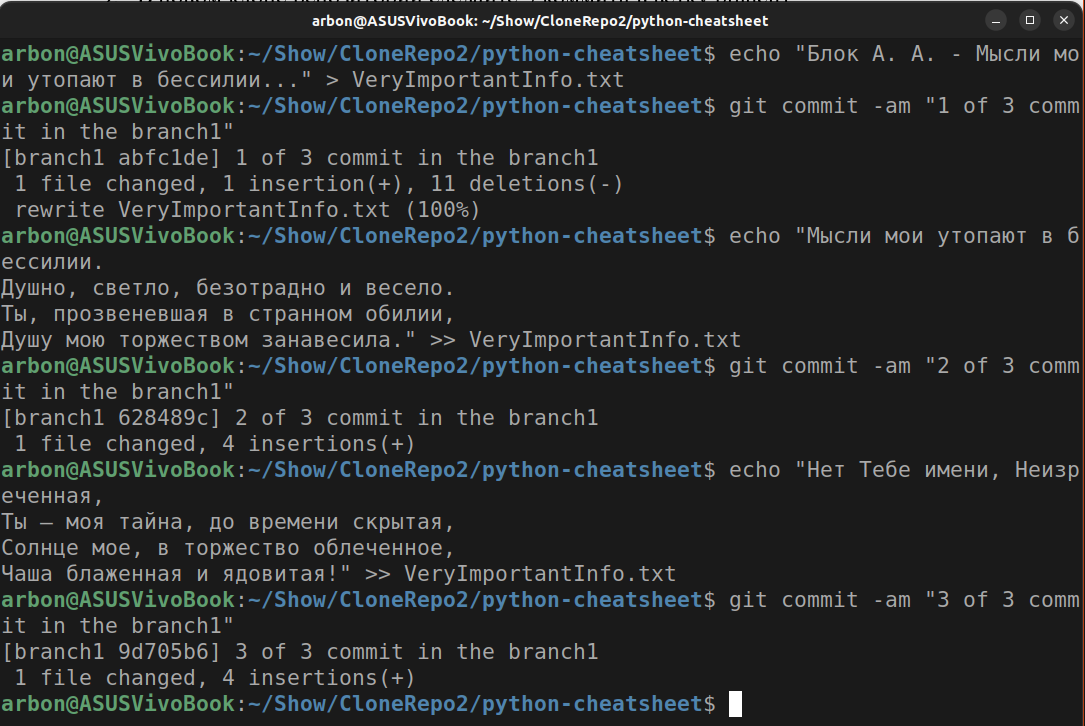
\includegraphics[width=0.7\textwidth]{Screenshot from 2023-02-20 12-11-45.png}
	\caption{Три коммита в новом репозитории}
	\label{3:fig:git:clone:new:commits}
\end{figure}

\section{Отправка изменнеий из нового репозитория}
Выгрузим все изменения из нового в удаленный репозиторий
(Рисунок~\ref{3:fig:git:clone:new:push}).

\begin{figure}[h!tp]
	\centering
	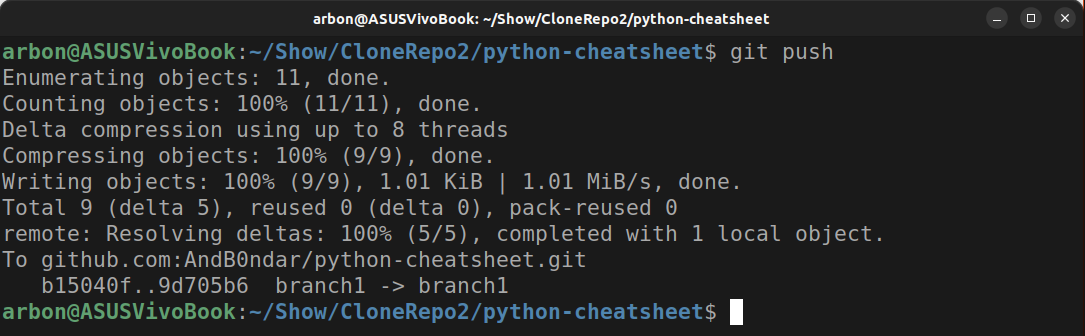
\includegraphics[width=0.7\textwidth]{Screenshot from 2023-02-20 12-12-56.png}
	\caption{Выгрузка изменений из нового репозитория}
	\label{3:fig:git:clone:new:push}
\end{figure}

\section{Отправка изменнеий из старого репозитория}
Вернемся в старый клон с репозиторием и выгрузим изменения
с опцией \verb|--force| (Рисунок~\ref{3:fig:git:clone:push}).

\begin{figure}[h!tp]
	\centering
	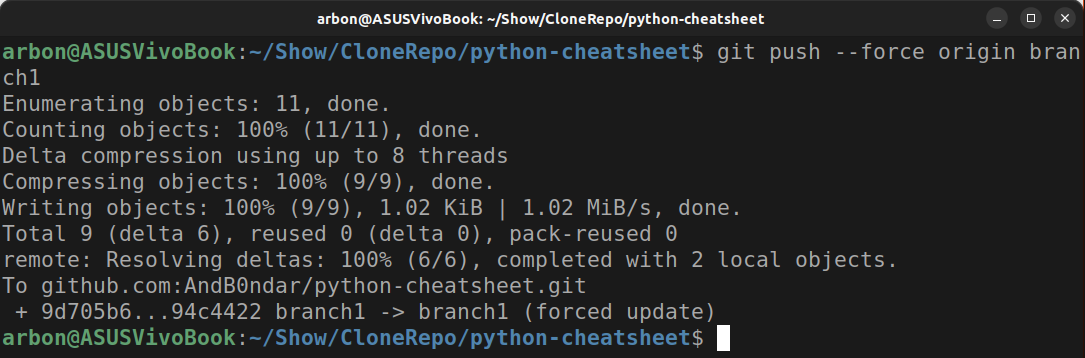
\includegraphics[width=0.7\textwidth]{Screenshot from 2023-02-20 12-18-32.png}
	\caption{Выгрузка изменений из старого репозитория}
	\label{3:fig:git:clone:push}
\end{figure}

\section{Разрешение конфликта слияния веток}
Теперь получим все изменения в новом репозитории.
При попытке вытягивания с помощью команды \texttt{git~pull}, git выдал
ошибку из-за конфликта слияния веток и предложил три метода решения:
\begin{verbatim}
	git config pull.rebase false  # merge (the default strategy)
	git config pull.rebase true   # rebase
	git config pull.ff only       # fast-forward only
\end{verbatim}
Введя одну из команд, снова вводим команду вытягивания. Затем устранияем
конфилкт слияния, также как это делалось
выше~(см.~стр.~\pageref{3:lb:git:merge:conflict}).
Вывод команд показан на рисунке~\ref{3:fig:git:clone:new:pull}.

\begin{figure}[h!tp]
	\centering
	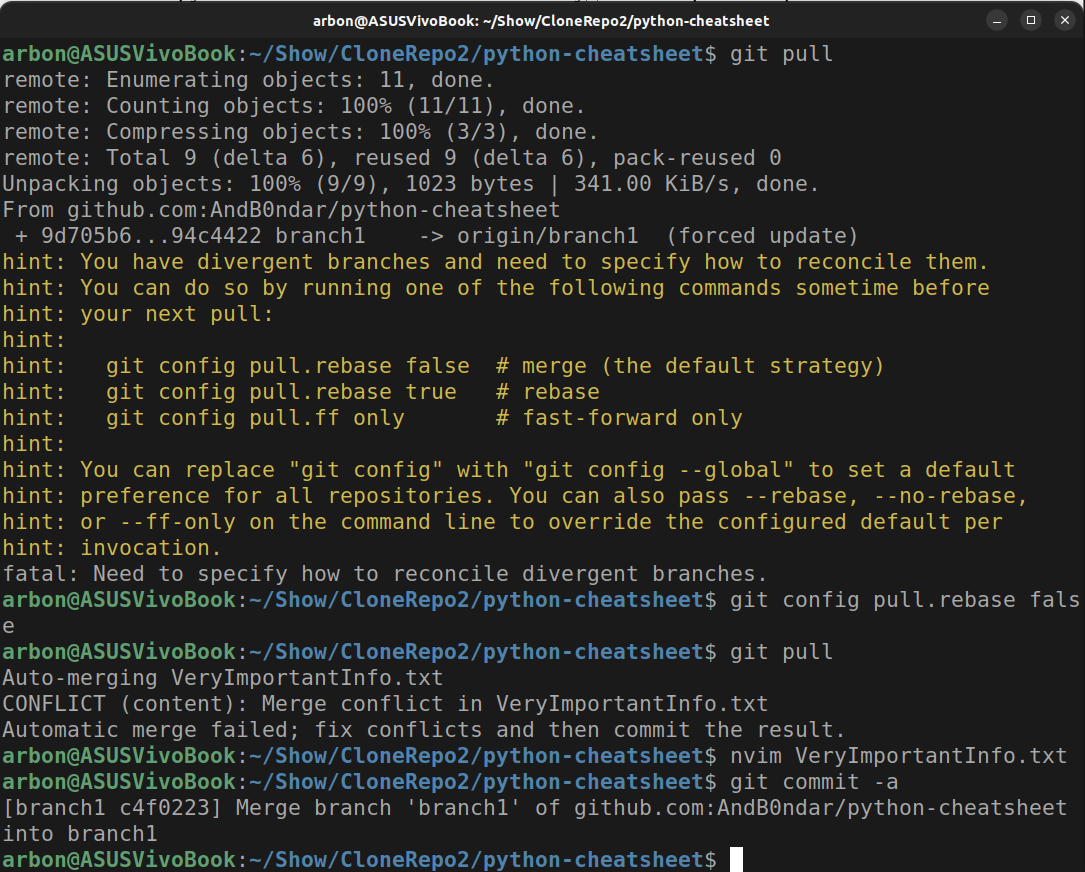
\includegraphics[width=0.8\textwidth]{Screenshot from 2023-02-20 12-27-34.png}
	\caption{Вытягивание изменений в новый клон репозитория}
	\label{3:fig:git:clone:new:pull}
\end{figure}
